\documentclass[12pt]{article}

\usepackage{amsmath,amssymb}
\usepackage{geometry}
\geometry{margin=1.1in}
\usepackage{hyperref}
\usepackage{xcolor}
\usepackage{tcolorbox}
\usepackage{graphicx}
\usepackage{tikz}
\usetikzlibrary{arrows.meta,positioning,decorations.pathmorphing,calc}
\usepackage{booktabs}
\usepackage{enumitem}
\usepackage{microtype}

\tcbuselibrary{breakable,skins}

\newtcolorbox{idea}{
  colback=blue!4, colframe=blue!45,
  title=Key Idea, fonttitle=\bfseries, breakable,
  left=6pt, right=6pt}

\newtcolorbox{analogy}{
  colback=green!4, colframe=green!45,
  title=Analogy, fonttitle=\bfseries, breakable,
  left=6pt, right=6pt}

\newtcolorbox{punchline}{
  colback=orange!5, colframe=orange!60,
  title=The Punchline, fonttitle=\bfseries, breakable,
  left=6pt, right=6pt}

\newcommand{\cl}{{\rm cl}}
\newcommand{\q}{{\rm q}}
\newcommand{\Keldysh}{{\rm K}}
\newcommand{\bra}[1]{\langle #1 |}
\newcommand{\ket}[1]{| #1 \rangle}
\newcommand{\braket}[2]{\langle #1 | #2 \rangle}
\newcommand{\av}[1]{\langle #1 \rangle}
\providecommand{\cl}{{\rm cl}}
\providecommand{\q}{{\rm q}}
\providecommand{\Keldysh}{{\rm K}}

\begin{document}

\title{\textbf{Path Integrals and the Keldysh Formalism}\\[0.4em]
\large A Plain-Language Guide for Beginning PhD Students}

\author{Notes prepared as a companion to the QNM paper}
\date{}
\maketitle
\tableofcontents
\newpage

%----------------------------------------------------------------------
\section{Before We Start: What We Are Trying to Do}
%----------------------------------------------------------------------

You have probably seen the Schrödinger equation. You know that quantum
mechanics is about wavefunctions and operators and expectation values.
That is the \emph{wavefunction picture}.

This tutorial introduces a completely different way of organizing the
same physics: the \emph{path integral picture}, developed by Richard
Feynman in the 1940s. Then we introduce the \emph{Keldysh formalism},
which extends path integrals to systems that exchange energy with their
environment --- like a laser cavity leaking photons, or an atom
spontaneously emitting light.

By the end you should understand why the main paper is structured the
way it is, what all the symbols mean, and why the method works.

\begin{idea}
The wavefunction picture and the path integral picture are two
ways of computing the same thing. Neither is ``more correct.''
The path integral is often much easier to use when the system has
many interacting parts or is coupled to a large environment.
\end{idea}

%----------------------------------------------------------------------
\section{A Quick Reminder: What Quantum Mechanics Is About}
%----------------------------------------------------------------------

\subsection{States, operators, and probabilities}

In quantum mechanics a \textbf{state} $\ket{\psi}$ is a complete
description of what you know about a physical system. If you measure
an observable $\hat{O}$ (position, energy, photon number, etc.), you
do not necessarily get a single definite answer --- you get a random
outcome drawn from some probability distribution. The average of many
such measurements is the \textbf{expectation value}:
\begin{equation}
  \av{\hat{O}} = \bra{\psi}\hat{O}\ket{\psi}
\end{equation}

\subsection{Time evolution}

States evolve in time according to the Schrödinger equation:
\begin{equation}
  i\hbar\frac{d}{dt}\ket{\psi(t)} = \hat{H}\ket{\psi(t)}
\end{equation}
The formal solution is $\ket{\psi(t)} = e^{-i\hat{H}t/\hbar}\ket{\psi(0)}$.
The operator $\hat{U}(t) = e^{-i\hat{H}t/\hbar}$ is the
\textbf{time evolution operator}.

\subsection{The key formula we want to compute}

Everything we care about in quantum physics can be expressed as:
\begin{equation}
  \av{\hat{O}(t)} = \bra{\psi(0)}\hat{U}^\dagger(t)\,\hat{O}\,\hat{U}(t)\ket{\psi(0)}
  \label{eq:expect}
\end{equation}
The path integral is a clever way to compute \emph{this formula}
without explicitly finding the wavefunction.

%----------------------------------------------------------------------
\section{The Feynman Path Integral: The Basic Idea}
%----------------------------------------------------------------------

\subsection{The two-slit experiment as intuition}

In the famous two-slit experiment, a particle can go through either
slit to reach a detector. The quantum rule is:
\begin{itemize}
  \item Assign each path a complex number (an \emph{amplitude}).
  \item Add up the amplitudes for all paths.
  \item The probability is the square of the total amplitude.
\end{itemize}

Feynman's insight was to generalize this: \textbf{every} quantum
amplitude can be written as a sum over \emph{all} possible paths,
not just two.

\begin{figure}[h]
\centering
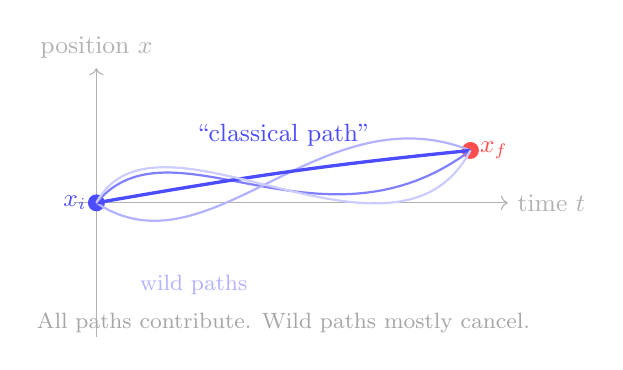
\begin{tikzpicture}[scale=0.95]
  % axes
  \draw[->,gray!60] (-0.3,0) -- (5.5,0) node[right,font=\small]{time $t$};
  \draw[->,gray!60] (0,-1.8) -- (0,1.8) node[above,font=\small]{position $x$};
  % start and end points
  \filldraw[blue!70] (0,0) circle (3pt) node[left,font=\small]{$x_i$};
  \filldraw[red!70] (5,0.7) circle (3pt) node[right,font=\small]{$x_f$};
  % various paths
  \draw[blue!50, thick] (0,0) .. controls (1,1.2) and (3,-0.8) .. (5,0.7);
  \draw[blue!30, thick] (0,0) .. controls (1.5,-1.0) and (3,1.5) .. (5,0.7);
  \draw[blue!70, very thick] (0,0) .. controls (2,0.35) and (3,0.5) .. (5,0.7);
  \draw[blue!20, thick] (0,0) .. controls (0.8,1.5) and (4,-1.2) .. (5,0.7);
  % labels
  \node[blue!70,font=\small] at (2.5,0.9) {``classical path''};
  \node[blue!30,font=\footnotesize] at (1.3,-1.1) {wild paths};
  \node[font=\footnotesize,gray!70] at (2.5,-1.6)
    {All paths contribute. Wild paths mostly cancel.};
\end{tikzpicture}
\caption{In the path integral, a particle travels from $x_i$ to $x_f$ by
following \emph{all} possible paths simultaneously, each weighted by a phase
$e^{iS[\text{path}]/\hbar}$.}
\end{figure}

\subsection{The action: the weight of each path}

Each path gets a weight $e^{iS[\text{path}]/\hbar}$, where
$S$ is the \textbf{action} of that path:
\begin{equation}
  S[\text{path}] = \int_{t_i}^{t_f} dt\;
  \underbrace{L(x(t), \dot{x}(t))}_{\text{Lagrangian}}
\end{equation}
For a particle with mass $m$ in a potential $V(x)$:
\begin{equation}
  L = \underbrace{\frac{1}{2}m\dot{x}^2}_{\text{kinetic}} -
  \underbrace{V(x)}_{\text{potential}}
\end{equation}

The key observation: \textbf{the classical path is the path that
makes $S$ stationary} (i.e., $\delta S = 0$). This is just the
principle of stationary action from classical mechanics. Quantum
mechanics says all paths contribute, but wild paths have rapidly
oscillating phases $e^{iS/\hbar}$ that cancel each other --- the
classical path ``wins'' because its neighbors all have similar phases
and add up constructively.

\begin{analogy}
Imagine many friends all walking from your home to a coffee shop
by different routes, each twirling a clock hand as they walk at a
rate proportional to their path length. When they arrive, you add
up all their clock vectors. The direct route and its nearby variants
all arrive with clock hands pointing in roughly the same direction
and add constructively. The wildly indirect routes arrive with
clock hands pointing in random directions and cancel. The most
probable path is the direct one --- this is the classical path.
\end{analogy}

\subsection{The path integral formula}

The quantum amplitude for going from state $\ket{x_i}$ to state
$\ket{x_f}$ in time $T$ is:
\begin{equation}
  \bra{x_f}\hat{U}(T)\ket{x_i} =
  \int_{\text{all paths}} \mathcal{D}[x(t)]\;e^{iS[x(t)]/\hbar}
  \label{eq:path_integral}
\end{equation}
where $\int\mathcal{D}[x(t)]$ means ``sum over all paths starting
at $x_i$ and ending at $x_f$.'' This is a formal expression ---
making it mathematically precise requires some care --- but it
captures all of quantum mechanics.

\begin{punchline}
The path integral is nothing mysterious: it is just another way to
compute $\bra{x_f}e^{-i\hat{H}T/\hbar}\ket{x_i}$. It is useful
because we can often do the integral over paths more easily than
we can diagonalize the Hamiltonian $\hat{H}$.
\end{punchline}

%----------------------------------------------------------------------
\section{From Particles to Fields: Second Quantization in One Page}
%----------------------------------------------------------------------

\subsection{Why we need ``second quantization''}

In quantum optics we do not talk about the position of a single
particle. We talk about \emph{photon modes} --- electromagnetic field
modes each of which can contain 0, 1, 2, \ldots photons.

A single mode (say, the mode of a cavity at frequency $\omega_0$) is
described by:
\begin{itemize}
  \item $\hat{a}$: the \textbf{annihilation operator} (removes one photon)
  \item $\hat{a}^\dagger$: the \textbf{creation operator} (adds one photon)
  \item $\hat{n} = \hat{a}^\dagger\hat{a}$: the photon number operator
\end{itemize}
These satisfy $[\hat{a}, \hat{a}^\dagger] = 1$ (the canonical
commutation relation for bosons).

The state with exactly $n$ photons is $\ket{n}$, and:
$\hat{a}\ket{n} = \sqrt{n}\ket{n-1}$,
$\hat{a}^\dagger\ket{n} = \sqrt{n+1}\ket{n+1}$.

\subsection{Coherent states: the bridge to classical fields}

A \textbf{coherent state} $\ket{\alpha}$ (where $\alpha\in\mathbb{C}$)
is an eigenstate of the annihilation operator:
\begin{equation}
  \hat{a}\ket{\alpha} = \alpha\ket{\alpha}
\end{equation}
A coherent state is the quantum state that behaves most like a
classical oscillating field: the electric field has a definite
amplitude $\propto\mathrm{Re}(\alpha e^{-i\omega_0 t})$ with small
quantum fluctuations. A laser far above threshold produces a coherent state.

Coherent states are complete: $\int d^2\alpha/\pi\,\ket{\alpha}\bra{\alpha} = \mathbf{1}$.
This completeness relation is the key that lets us write path integrals
for quantum fields.

\begin{idea}
In the path integral for a field mode, the c-number $\alpha(t)$
--- the coherent-state eigenvalue --- plays the role of the
``position'' $x(t)$ in the particle path integral. At each
moment of time, the state of the mode is described by a complex
number $\alpha(t)$, and we integrate over all possible histories
$\{\alpha(t)\}$.
\end{idea}

%----------------------------------------------------------------------
\section{The Path Integral for a Quantum Field Mode}
%----------------------------------------------------------------------

\subsection{Building the action}

Insert the coherent-state resolution of the identity at many time
steps between $t_i$ and $t_f$. At each step, the overlap of
neighboring coherent states gives:
$\bra{\alpha(t+\delta t)}\alpha(t)\rangle \approx
e^{\alpha^*(t+\delta t)\partial_t\alpha(t)\,\delta t}$.

Collecting all steps, the path integral for a single cavity mode
with Hamiltonian $\hat{H} = \hbar\omega_0\hat{a}^\dagger\hat{a}$:
\begin{equation}
  \bra{\alpha_f}\hat{U}(T)\ket{\alpha_i} =
  \int\mathcal{D}[\alpha^*(t),\alpha(t)]\;e^{iS[\alpha^*,\alpha]/\hbar}
\end{equation}
\begin{equation}
  S = \int_{t_i}^{t_f} dt\,\hbar\Bigl[
  \underbrace{i\alpha^*(t)\partial_t\alpha(t)}_{\text{Berry phase}}
  - \underbrace{\omega_0|\alpha(t)|^2}_{\text{energy}}
  \Bigr]
  \label{eq:action_field}
\end{equation}

The two terms:

\textbf{The Berry phase} $i\alpha^*\partial_t\alpha$: this
first-order kinetic term has no analogue in classical mechanics.
It is the path-integral encoding of $[\hat{a},\hat{a}^\dagger]=1$.
If you removed this term, $\alpha(t)$ would just be a classical
variable with no quantum noise.

\textbf{The energy} $-\omega_0|\alpha|^2$: this is the classical
energy of the oscillator, $\hbar\omega_0\times(\text{amplitude squared})$.

\subsection{The saddle point: recovering classical physics}

The saddle point of $S$ is the path where $\delta S/\delta\alpha^* = 0$:
\begin{equation}
  i\partial_t\alpha = \omega_0\alpha
  \quad\Rightarrow\quad
  \alpha(t) = \alpha_i\,e^{-i\omega_0 t}
\end{equation}
This is just the classical oscillation! The saddle point always
gives the \emph{classical equations of motion}. Quantum mechanics
comes from integrating over all the non-saddle-point paths
(the fluctuations around the classical path).

%----------------------------------------------------------------------
\section{Open Systems: The Problem of the Environment}
%----------------------------------------------------------------------

\subsection{Why open systems need special treatment}

A real cavity leaks photons. The cavity field $\hat{a}$ couples to
an environment (the electromagnetic vacuum outside the cavity, or a
thermal bath), exchanging energy continuously.

The quantum state of the \emph{system + environment} evolves
unitarily. But we are only interested in the system (the cavity
mode). When we ``trace out'' the environment --- sum over all
environmental states --- we get the \emph{reduced density matrix}
$\rho_{\rm sys}(t)$.

The expectation value of any observable is:
\begin{equation}
  \av{\hat{O}(t)} = \mathrm{Tr}[\rho_{\rm sys}(t)\hat{O}]
  = \mathrm{Tr}\bigl[\hat{U}(t)\rho_0\hat{U}^\dagger(t)\hat{O}\bigr]
  \label{eq:open_expect}
\end{equation}
There is a \emph{forward} evolution $\hat{U}$ and a \emph{backward}
evolution $\hat{U}^\dagger$. This is the core problem for open systems:
a single path integral only goes one way in time.

\begin{figure}[h]
\centering
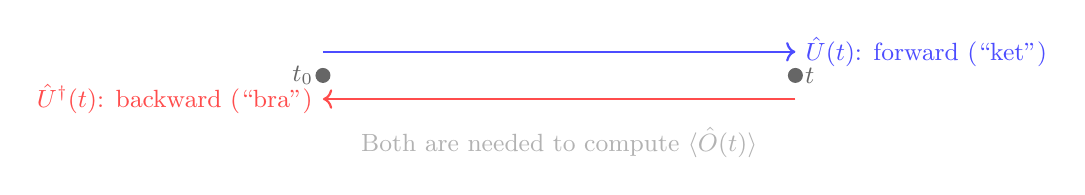
\begin{tikzpicture}[scale=1.0]
  \draw[->,thick,blue!70] (-3,0.3) -- (3,0.3)
    node[right,font=\small,blue!70] {$\hat{U}(t)$: forward (``ket'')};
  \draw[->,thick,red!70] (3,-0.3) -- (-3,-0.3)
    node[left,font=\small,red!70] {$\hat{U}^\dagger(t)$: backward (``bra'')};
  \filldraw[black!60] (-3,0) circle (2.5pt)
    node[left,font=\small]{$t_0$};
  \filldraw[black!60] (3,0) circle (2.5pt)
    node[right,font=\small]{$t$};
  \node[font=\small,gray!60] at (0,-0.85)
    {Both are needed to compute $\av{\hat{O}(t)}$};
\end{tikzpicture}
\caption{Computing $\av{\hat{O}(t)} = \mathrm{Tr}[\hat{U}\rho_0\hat{U}^\dagger\hat{O}]$
requires propagating forward in time (for $\hat{U}$, the ``ket'')
and backward in time (for $\hat{U}^\dagger$, the ``bra'').}
\end{figure}

%----------------------------------------------------------------------
\section{The Keldysh Trick: Two Time Branches}
%----------------------------------------------------------------------

\subsection{The closed-time-path contour}

Schwinger (1961) and Keldysh (1965) solved the open-system problem
by \textbf{doubling the time contour}: go forward from $t_0$ to $t$,
then come back from $t$ to $t_0$. This ``closed time path'' (CTP) is
drawn in Fig.~\ref{fig:CTP}.

\begin{figure}[h]
\centering
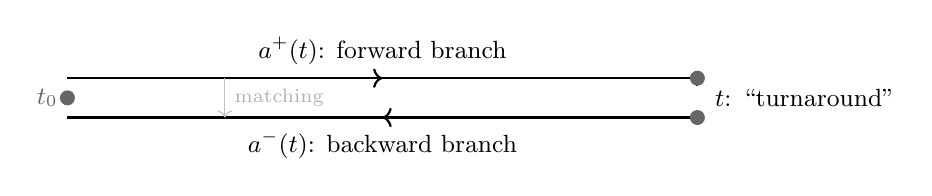
\begin{tikzpicture}[scale=1.0]
  \draw[->,thick] (-4,0) -- (0,0);
  \draw[thick] (-4,0) -- (4,0) -- (4,-0.1);
  \draw[->,thick] (4,-0.5) -- (0,-0.5);
  \draw[thick] (4,-0.5) -- (-4,-0.5);
  % arrows and labels
  \node[font=\small] at (0,0.35) {$a^+(t)$: forward branch};
  \node[font=\small] at (0,-0.85) {$a^-(t)$: backward branch};
  \filldraw[black!60] (-4,-0.25) circle (2.5pt)
    node[left,font=\small]{$t_0$};
  \filldraw[black!60] (4,0) circle (2.5pt);
  \filldraw[black!60] (4,-0.5) circle (2.5pt);
  \node[right,font=\small] at (4.1,-0.25) {$t$: ``turnaround''};
  \draw[gray!50,->] (-2,0) -- (-2,-0.5)
    node[midway,right,font=\scriptsize,gray!60]{matching};
\end{tikzpicture}
\caption{The Keldysh closed-time-path (CTP) contour.  The field $a^+(t)$
lives on the forward branch (corresponding to $\hat{U}$) and $a^-(t)$ lives
on the backward branch (corresponding to $\hat{U}^\dagger$).  At the
``turnaround'' time $t$, forward and backward branches are joined.
The path integral over both branches computes $\mathrm{Tr}[\hat{U}\rho_0
\hat{U}^\dagger\hat{O}]$ exactly.}
\label{fig:CTP}
\end{figure}

The \textbf{Keldysh path integral} introduces two c-number fields:
\begin{itemize}
  \item $a^+(t)$: the coherent-state field on the \textbf{forward} branch
    (carries the ``ket'' information from $\hat{U}$)
  \item $a^-(t)$: the coherent-state field on the \textbf{backward} branch
    (carries the ``bra'' information from $\hat{U}^\dagger$)
\end{itemize}
and computes:
\begin{equation}
  \av{\hat{O}(t)} =
  \int\mathcal{D}[a^\pm]\,O[a^+,a^-]\,
  e^{iS[a^+] - iS^*[a^-]}
  \label{eq:Keldysh_PI}
\end{equation}

\begin{analogy}
Think of a movie with two simultaneous ``cuts'': the official
version (forward branch, $a^+$) and the director's cut
(backward branch, $a^-$). Computing $\av{\hat{O}}$ requires
watching both cuts at once and comparing them. In classical
physics the two cuts are identical. In quantum mechanics they
can differ --- the difference is quantum noise.
\end{analogy}

\subsection{The classical-quantum rotation}

Instead of $a^+$ and $a^-$, it is more convenient to work with
their sum and difference:
\begin{equation}
  \underbrace{a^\cl = \tfrac{1}{2}(a^+ + a^-)}_{\text{``classical field'': the average}},\quad
  \underbrace{a^\q = a^+ - a^-}_{\text{``quantum field'': the difference}}
  \label{eq:clq}
\end{equation}

\textbf{$a^\cl(t)$} is the average of forward and backward paths.
Its expectation value is the quantum mean field:
$\av{a^\cl} = \av{\hat{a}(t)}$.

\textbf{$a^\q(t)$} is the difference. In classical physics the
forward and backward paths are identical, so $a^\q = 0$. A
nonzero $a^\q$ is a purely quantum effect: it measures how much
the ``ket path'' and the ``bra path'' deviate from each other.

\begin{idea}
$a^\cl$ is what a classical instrument (a heterodyne detector)
would measure: the coherent amplitude. $a^\q$ is what a quantum
instrument would additionally reveal: the quantum fluctuations
that make the two branches differ. The fact that we need both
to describe an open quantum system is the heart of the Keldysh
formalism.
\end{idea}

%----------------------------------------------------------------------
\section{The Keldysh Action: The Single Most Important Formula}
%----------------------------------------------------------------------

\subsection{Writing the action in the cl-q basis}

For a single cavity mode coupled to a thermal bath at temperature $T$,
the Keldysh action in frequency space is:
\begin{equation}
  S_K = \int\frac{d\omega}{2\pi}
  \begin{pmatrix}a^{\cl*} & a^{\q*}\end{pmatrix}
  \underbrace{
  \begin{pmatrix}
    0 & \omega - \omega_0 - i\kappa/2\\
    \omega - \omega_0 + i\kappa/2 & -i\kappa(2\bar{n}+1)
  \end{pmatrix}
  }_{\text{the Keldysh matrix}}
  \begin{pmatrix}a^\cl\\a^\q\end{pmatrix}
  \label{eq:SK}
\end{equation}
where $\kappa$ is the cavity decay rate and $\bar{n} = 1/(e^{\hbar\omega_0/k_BT}-1)$
is the mean thermal photon number.

Let us read this matrix entry by entry:

\begin{center}
\begin{tabular}{ccc}
\toprule
Entry & Value & Physical meaning \\
\midrule
(1,1) & $0$ & Causality: $\av{a^\q a^{\q*}} = 0$ always \\
(1,2) $= [G^A]^{-1}$ & $\omega - \omega_0 - i\kappa/2$ & Advanced (bra) propagator \\
(2,1) $= [G^R]^{-1}$ & $\omega - \omega_0 + i\kappa/2$ & Retarded (ket) propagator \\
(2,2) $= D^\Keldysh$ & $-i\kappa(2\bar{n}+1)$ & Noise kernel \\
\bottomrule
\end{tabular}
\end{center}

\subsection{Physical meaning of each entry}

\textbf{The (2,1) entry}, $[G^R]^{-1} = \omega - \omega_0 + i\kappa/2$:
its inverse is the retarded Green's function
$G^R(\omega) = 1/(\omega - \omega_0 + i\kappa/2)$.
This is the Lorentzian lineshape you see on a spectrum analyser when
you drive the cavity with a probe: the cavity \emph{responds} to a
probe at frequency $\omega$ with amplitude $G^R(\omega)$.

\textbf{The (1,2) entry} $[G^A]^{-1}$ is just the complex conjugate of
$[G^R]^{-1}$. No new physics.

\textbf{The (2,2) entry} $D^\Keldysh = -i\kappa(2\bar{n}+1)$: this is
the \emph{noise kernel}. It tells you how much noise the environment
injects into the cavity. At zero temperature ($\bar{n}=0$):
$D^\Keldysh = -i\kappa$ --- vacuum fluctuations. At high temperature:
$D^\Keldysh \approx -2i\kappa\bar{n}$ --- thermal noise.

\textbf{The (1,1) entry is zero.} This is not an approximation --- it
is an exact consequence of the structure of quantum mechanics.
$\av{a^\q a^{\q*}} = 0$ encodes the identity $\mathrm{Tr}[\rho U^\dagger U] = 1$.
If this entry were nonzero, probability would not be conserved.

\subsection{The propagators: what you can read off immediately}

Inverting the $2\times 2$ Keldysh matrix gives the three propagators:
\begin{align}
  G^R(\omega) &= \frac{1}{\omega-\omega_0+i\kappa/2}
  \quad\text{(cavity response)} \\
  G^A(\omega) &= \frac{1}{\omega-\omega_0-i\kappa/2}
  \quad\text{(complex conjugate)} \\
  G^\Keldysh(\omega) &= G^R(\omega)\cdot D^\Keldysh\cdot G^A(\omega)
  = \frac{-i\kappa(2\bar{n}+1)}{|\omega-\omega_0|^2+(\kappa/2)^2}
  \quad\text{(noise spectrum)}
\end{align}

\begin{punchline}
$G^\Keldysh(\omega)$ is the \textbf{output noise power spectrum}
of the cavity --- the thing a spectrum analyser measures when
the cavity is in thermal equilibrium. Its value at resonance
($\omega = \omega_0$) gives the photon number:
$\bar{n} = (-iG^\Keldysh_{\omega=\omega_0}\cdot\kappa/4) - 1/2$.
The Keldysh formalism computes noise spectra as naturally as
$G^R$ computes response.
\end{punchline}

%----------------------------------------------------------------------
\section{The Fluctuation-Dissipation Theorem Falls Out for Free}
%----------------------------------------------------------------------

You may know the fluctuation-dissipation theorem (FDT): the noise
in a system in thermal equilibrium is related to its response by:
\begin{equation}
  \text{noise} = \text{response} \times \text{occupation}
\end{equation}
In Keldysh language this is exactly:
\begin{equation}
  G^\Keldysh(\omega) = (G^R(\omega) - G^A(\omega))\cdot(2\bar{n}+1)
  \label{eq:FDT_K}
\end{equation}
This follows automatically from the structure of $S_K$. You do not
need to assume it --- the path integral \emph{derives} it.

In a system \emph{out of equilibrium} (a laser above threshold,
a driven cavity, a gain medium), this relation breaks down. The
Keldysh formalism handles non-equilibrium systems by allowing
$D^\Keldysh$ to take values that are not consistent with a
Boltzmann distribution. This is exactly what happens with gain:
the gain bath contributes $+ig(2N_{\rm sp}+1)$, which has the
\emph{opposite sign} from the loss bath $-i\kappa(2n+1)$.

%----------------------------------------------------------------------
\section{How the Equations of Motion Come Out}
%----------------------------------------------------------------------

\subsection{The saddle point equation}

To find the most probable field amplitude $a^\cl(t)$, we minimize the
action --- set its variation to zero:
\begin{equation}
  \frac{\delta S_K}{\delta a^{\q*}(\omega)} = 0
  \quad\Rightarrow\quad
  \bigl(\omega - \omega_0 + i\kappa/2\bigr)\,a^\cl(\omega) = 0
\end{equation}
In the time domain:
\begin{equation}
  \frac{da^\cl}{dt} = \bigl(-i\omega_0 - \kappa/2\bigr)\,a^\cl
  \label{eq:EOM}
\end{equation}
This says: the cavity amplitude decays at rate $\kappa/2$ while
oscillating at frequency $\omega_0$. \textbf{This is your ordinary
cavity equation of motion} --- it came out of varying the Keldysh action.

\subsection{Adding the noise: the Langevin equation}

Equation \eqref{eq:EOM} is deterministic and has no noise.
The noise enters when we integrate out the quantum field $a^\q$.
The (2,2) entry $D^\Keldysh = -i\kappa(2\bar{n}+1)$ acts as a source
of stochastic forcing. After the integration, the equation for
$a^\cl$ becomes:
\begin{equation}
  \frac{da^\cl}{dt} =
  \bigl(-i\omega_0 - \kappa/2\bigr)a^\cl + \xi(t)
  \label{eq:Langevin}
\end{equation}
where $\xi(t)$ is a Gaussian random noise with:
\begin{align}
  \av{\xi^*(t)\xi(t')} &= \kappa\bar{n}\,\delta(t-t')
  \quad\text{(stimulated: photons come in)}\\
  \av{\xi(t)\xi^*(t')} &= \kappa(\bar{n}+1)\,\delta(t-t')
  \quad\text{(spontaneous + stimulated)}
\end{align}

\begin{punchline}
Equation \eqref{eq:Langevin} is \emph{exactly} the stochastic
Langevin equation you would write down from quantum input-output
theory. The Keldysh path integral derives it from scratch,
with the correct noise statistics, without any additional assumptions.
\end{punchline}

%----------------------------------------------------------------------
\section{Adding Nonlinearity: Feynman Diagrams}
%----------------------------------------------------------------------

\subsection{What nonlinearity does to the action}

A Kerr nonlinearity $\hat{H}_{\rm Kerr} = g^{(3)}\hat{a}^\dagger\hat{a}^\dagger\hat{a}\hat{a}$
adds quartic terms to the action. In the cl-q basis the most important one is:
\begin{equation}
  S_{\rm Kerr} \supset
  2g^{(3)}|a^\cl|^2\bigl(a^{\cl*}a^\q + a^{\q*}a^\cl\bigr)
  \label{eq:Kerr_vertex}
\end{equation}
This is a \textbf{vertex}: it describes the coupling between the
mean-field amplitude and the fluctuations.

\subsection{Feynman diagrams = organized perturbation theory}

When we compute $\av{\hat{O}}$ from the path integral with a
nonlinear action, we expand $e^{iS_{\rm Kerr}}$ in a Taylor series
in $g^{(3)}$. Each term in the series corresponds to a Feynman diagram.

\begin{figure}[h]
\centering
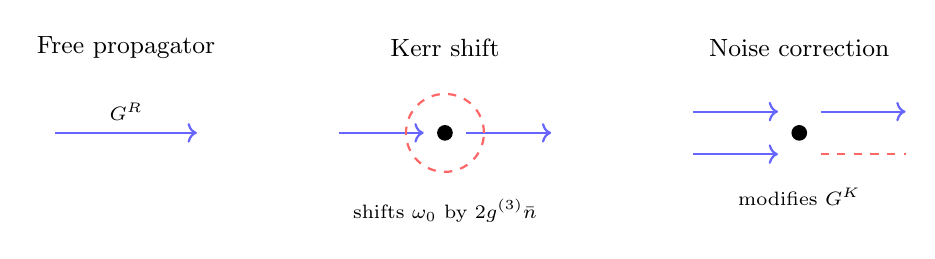
\begin{tikzpicture}[scale=0.9,
  line/.style={thick,blue!60},
  vertex/.style={circle,fill=black,inner sep=2pt},
  noisy/.style={thick,red!60,dashed}
]
%--- diagram 1: free propagator ---
\begin{scope}[xshift=-4.5cm]
  \node[font=\small] at (0,1.2) {Free propagator};
  \draw[line,->] (-1,0) -- (1,0);
  \node[font=\scriptsize] at (0,0.3) {$G^R$};
\end{scope}
%--- diagram 2: Kerr frequency shift ---
\begin{scope}[xshift=0cm]
  \node[font=\small] at (0,1.2) {Kerr shift};
  \draw[line,->] (-1.5,0) -- (-0.3,0);
  \node[vertex] (v) at (0,0) {};
  \draw[line,->] (0.3,0) -- (1.5,0);
  % loop
  \draw[noisy] (v) circle (0.55cm);
  \node[font=\scriptsize] at (0,-1.1) {shifts $\omega_0$ by $2g^{(3)}\bar{n}$};
\end{scope}
%--- diagram 3: noise correction ---
\begin{scope}[xshift=5cm]
  \node[font=\small] at (0,1.2) {Noise correction};
  \draw[line,->] (-1.5,0.3) -- (-0.3,0.3);
  \draw[line,->] (-1.5,-0.3) -- (-0.3,-0.3);
  \node[vertex] (v2) at (0,0) {};
  \draw[line,->] (0.3,0.3) -- (1.5,0.3);
  \draw[noisy] (0.3,-0.3) -- (1.5,-0.3);
  \node[font=\scriptsize] at (0,-0.9) {modifies $G^K$};
\end{scope}
\end{tikzpicture}
\caption{Feynman diagrams for a Kerr nonlinearity.  Solid lines are
retarded propagators $G^R$.  Dashed lines are Keldysh (noise)
propagators $G^K$.  Each vertex (dot) is a factor of $g^{(3)}$.
The ``tadpole'' diagram (middle) shifts the resonance frequency.
The box diagram (right) modifies the photon number statistics.}
\end{figure}

\subsection{Tree level vs loops: a hierarchy}

\textbf{Tree level} (no loops, no closed loops of propagator lines):
gives the classical mean field. If you drive a cavity and ask ``what
is the steady-state field amplitude?'', the answer is tree-level.

\textbf{One loop} (one closed loop): gives corrections of order
$\hbar$ to the classical result --- the leading quantum effects.
The laser linewidth, the photon number, the output noise spectrum:
all are one-loop quantities.

\textbf{Two loops}: gives corrections of order $\hbar^2$.
Higher-order photon statistics, $g^{(2)}(0)$, squeezing corrections.

\textbf{All loops}: the full quantum answer.  Usually impractical
to compute analytically, but can be done numerically.

\begin{analogy}
Tree-level = treating the system like billiard balls (classical).
One loop = adding the leading quantum ``fuzziness'' --- the
uncertainty principle and zero-point motion.
Two loops = adding the leading effect of interactions on the
quantum fuzziness.
\end{analogy}

%----------------------------------------------------------------------
\section{Gain Media: Why the Sign Flips}
%----------------------------------------------------------------------

\subsection{Loss vs. gain}

A loss bath (mirror transmission, absorption) extracts photons
from the cavity. In Keldysh language, it contributes a noise kernel:
\begin{equation}
  D^\Keldysh_{\rm loss} = -i\kappa(2\bar{n}+1) \leq 0
  \quad\text{at } T\geq 0
\end{equation}
This is always negative-imaginary for a passive loss bath.
Physically: loss \emph{damps} quantum fluctuations.

A gain medium (inverted two-level atoms) \emph{adds} photons to
the cavity. It contributes:
\begin{equation}
  D^\Keldysh_{\rm gain} = +ig(2N_{\rm sp}+1) \geq 0
\end{equation}
The opposite sign reflects the fundamental physical difference:
\textbf{gain amplifies vacuum fluctuations, while loss damps them}.

The total noise kernel:
\begin{equation}
  D^\Keldysh_{\rm total} =
  \underbrace{-i\kappa(2\bar{n}+1)}_{\text{loss, damps}} +
  \underbrace{+ig(2N_{\rm sp}+1)}_{\text{gain, amplifies}}
\end{equation}

At lasing threshold ($g=\kappa$, $T=0$, $N_{\rm sp}=1$):
$D^\Keldysh_{\rm total} = +2ig \neq 0$. The noise diverges as
$G^\Keldysh \propto D^\Keldysh/|G^R|^{-2}$ with $|G^R|^{-2}\to 0$.
This is the critical fluctuations of the laser threshold --- a
phase transition driven by amplified spontaneous emission noise.

%----------------------------------------------------------------------
\section{What the Full Framework Computes}
%----------------------------------------------------------------------

\subsection{A summary of what lives at each level}

\begin{center}
\begin{tabular}{lp{0.55\linewidth}}
\toprule
Keldysh level & Physical quantities \\
\midrule
Action $S_K$ & All dynamics encoded; read off $G^R$, $G^A$, $D^K$
  directly from the matrix entries \\
Saddle point & Mean-field: laser amplitude $\alpha_0$, comb amplitudes,
  threshold condition \\
One-loop ($G^K$) & Linewidth, photon number, squeezing spectrum, output
  noise, QFI for sensing \\
Two-loop & $g^{(2)}(0)$, Mandel $Q$, Kerr squeezing, parametric squeezing \\
All-loop (resummed) & Full photon statistics $P(n)$, photon blockade,
  non-Gaussian states \\
\bottomrule
\end{tabular}
\end{center}

\subsection{Why use this instead of the master equation?}

For a single mode with a few photons, the Lindblad master equation
is often simpler. The Keldysh formalism wins when:

\begin{enumerate}[leftmargin=1.5em]
  \item \textbf{Many modes.} A frequency comb has 100+ modes.
    The master equation Hilbert space scales as $n_{\rm max}^{100}$
    (impossibly large). The Keldysh path integral has 100 fields
    plus their interactions --- manageable.

  \item \textbf{Spatial structure.} The coupling constants
    $g^{(2,3)}_{\lambda\mu\nu}$ are overlap integrals of QNM mode
    functions in real space. The path integral makes this explicit;
    the master equation does not.

  \item \textbf{Topology optimization.} The gradient of any observable
    with respect to the structure geometry is computable from the
    Keldysh action using the adjoint method.

  \item \textbf{SALT integration.} The nonlinear lasing mode functions
    from SALT can be plugged directly into the Keldysh path integral
    as the basis, giving quantum noise for deeply nonlinear lasers.
\end{enumerate}

%----------------------------------------------------------------------
\section{The Complete Dictionary}
%----------------------------------------------------------------------

\begin{center}
\begin{tabular}{p{0.40\linewidth}p{0.50\linewidth}}
\toprule
Everyday language & Keldysh symbol \\
\midrule
``The cavity field amplitude'' & $a^\cl(t)$ or $\av{\hat{a}(t)}$ \\
``The cavity response curve'' & Retarded propagator $G^R(\omega)$ \\
``The output noise spectrum'' & Keldysh propagator $G^\Keldysh(\omega)$ \\
``Thermal noise in the cavity'' & $D^\Keldysh = -i\kappa(2\bar{n}+1)$ \\
``Spontaneous emission noise'' & $D^\Keldysh_{\rm gain} = +ig(2N_{\rm sp}+1)$ \\
``The steady-state laser field'' & Saddle point of $S_K$ \\
``Laser linewidth'' & Phase diffusion rate from $G^\Keldysh_{\rm phase}$ \\
``Two-mode squeezing'' & Anomalous propagator $F(\omega) = \av{a^\cl a^\cl}$ \\
``$g^{(2)}(0)=1$ for coherent light'' & One-loop Keldysh gives $g^{(2)}\approx 1$ \\
``Photon blockade'' & All-loop resummation needed \\
``Coupling constants $g^{(2,3)}$'' & Overlap integrals of QNM mode functions \\
``Forward branch'' & $a^+(t)$, corresponds to $\hat{U}$ \\
``Backward branch'' & $a^-(t)$, corresponds to $\hat{U}^\dagger$ \\
``Quantum field $a^\q$'' &
  $a^+(t) - a^-(t)$; nonzero only due to quantum fluctuations \\
\bottomrule
\end{tabular}
\end{center}

%----------------------------------------------------------------------
\section{The Minimum Needed to Read the Main Paper}
%----------------------------------------------------------------------

If you take away only five things from this tutorial:

\begin{enumerate}
  \item \textbf{The Keldysh path integral is quantum mechanics in the
    coherent-state basis.} The fields $a^\pm$, $a^\cl$, $a^\q$ are
    all c-numbers --- but the theory is fully quantum because of the
    Berry phase term $i\int a^*\partial_t a\,dt$ and the Keldysh
    structure.

  \item \textbf{The action matrix tells you everything.}
    The (2,1) entry gives $G^R$ (cavity response).
    The (2,2) entry $D^\Keldysh$ gives the noise (photon statistics).
    The (1,1) entry is always zero (causality).

  \item \textbf{The saddle point gives your HL equations.}
    Varying $S_K$ with respect to $a^{\q*}$ produces the equation
    of motion for $a^\cl = \av{\hat{a}}$ --- with noise from $D^\Keldysh$.

  \item \textbf{Gain and loss have opposite signs in $D^\Keldysh$.}
    Loss damps fluctuations ($-i\kappa$). Gain amplifies them ($+ig$).
    This is why the laser transition is a critical point.

  \item \textbf{Loops organize quantum corrections.}
    One loop = Gaussian (linewidths, squeezing).
    Two loops = photon statistics.
    All loops = photon blockade, non-Gaussian states.
\end{enumerate}

\bigskip
\noindent With these five points, every section of the main paper
should make sense at the conceptual level.

\end{document}
